
\documentclass{article}
\usepackage[utf8]{inputenc}

\title{Laboratorio04_CALIDAD_PRUEBAS_SOFTWARE}
\author{edwartbalcon }
\date{October 2020}

\usepackage[utf8]{inputenc}
\usepackage[spanish]{babel}
\usepackage{natbib}
\usepackage{graphicx}

\begin{document}

\title{Caratula}

\begin{titlepage}
\begin{center}
\begin{Large}
\textbf{UNIVERSIDAD PRIVADA DE TACNA} \\
\end{Large}
\vspace*{-0.025in}
\begin{figure}[htb]
\begin{center}

\includegraphics[width=6cm]{./images/logo_UPT}
\end{center}
\end{figure}
\vspace*{-0.025in}
\begin{Large}
\textbf{FACULTAD DE INGENIERIA} \\
\end{Large}
\vspace*{0.05in}
\begin{Large}
\textbf{Escuela Profesional de Ingeniería de Sistema} \\
\end{Large}


\vspace*{0.4in}

\vspace*{0.1in}
\begin{Large}
\textbf{Informe de laboratorio 01: Introducción a big data con Amazon EMR} \\
\end{Large}

\vspace*{0.3in}
\begin{Large}
\textbf{Curso: Base de datos II} \\
\end{Large}

\vspace*{0.3in}
\begin{Large}
\textbf{DOCENTE: Ing. Patrick Cuadros Quiroga} \\
\end{Large}

\vspace*{0.2in}
\vspace*{0.1in}
\begin{large}

\begin{Large}
\textbf{Alumno: Balcon Coahila, Edwart Juan\hfill	(2013046516) } \\
\end{Large}

\vspace*{0.15in}
\begin{Large}
\textbf{Tacna – Perú} \\
\end{Large}

\vspace*{0.05in}
\begin{Large}
\textbf{2020 } \\
\end{Large}

\end{large}
\end{center}

\end{titlepage}


\newpage

\section{ Configurar los requisitos previos para el clúster de ejemplo}

\textbf{1.1. Inicie Sesión en AWS Educate, dirigirse a la Consola de Admiistración}

    \begin{center}
		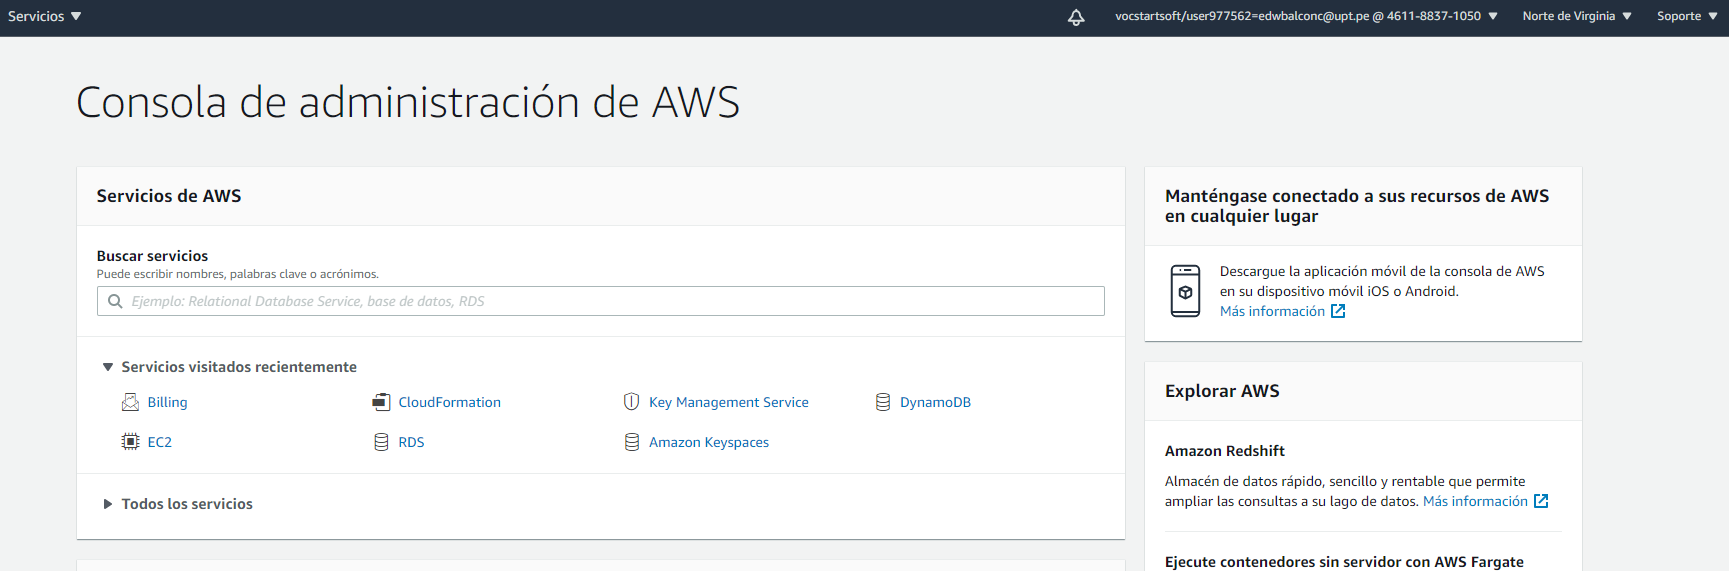
\includegraphics[width=15cm]{./images/1} 
	\end{center}
	
\textbf{1.2. Crear un bucket de Amazon S3}

    \begin{center}
		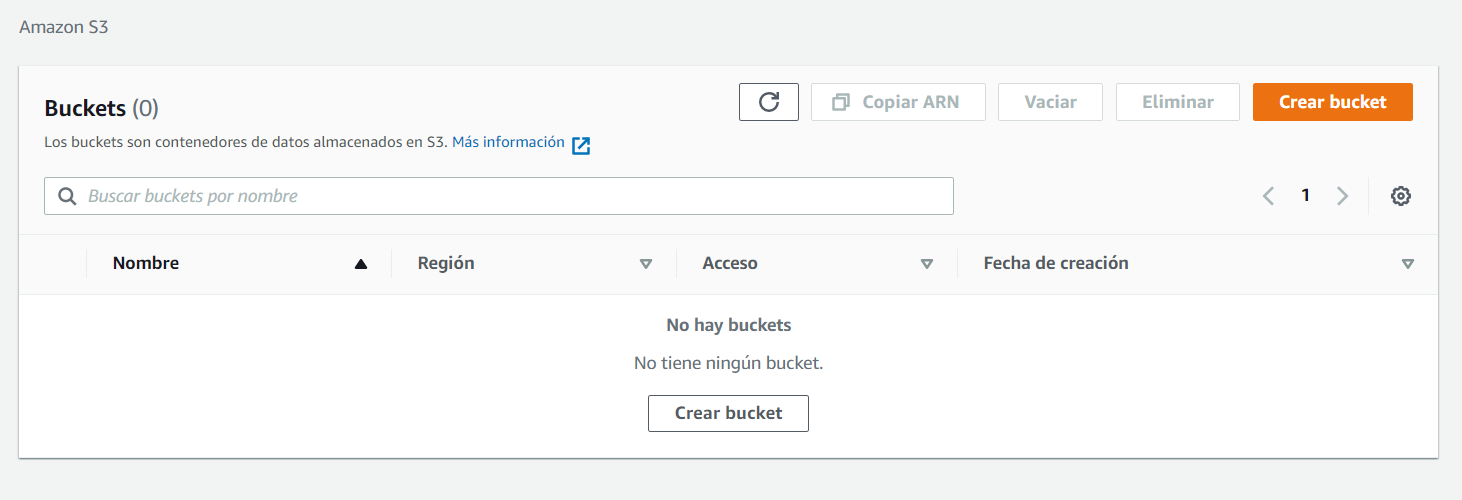
\includegraphics[width=15cm]{./images/2} 
	\end{center}
	\begin{center}
		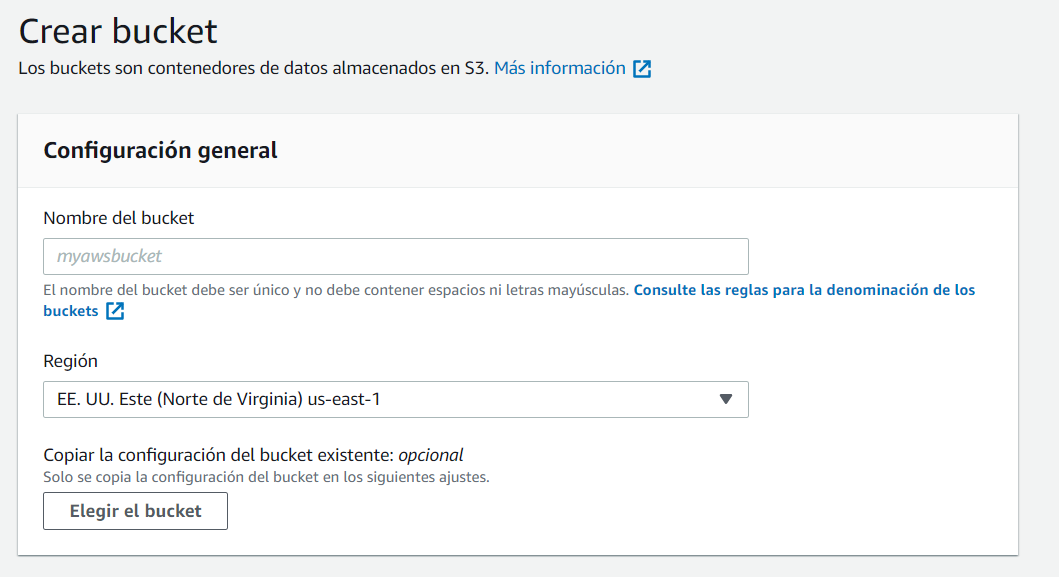
\includegraphics[width=15cm]{./images/3} 
	\end{center}
	\begin{center}
		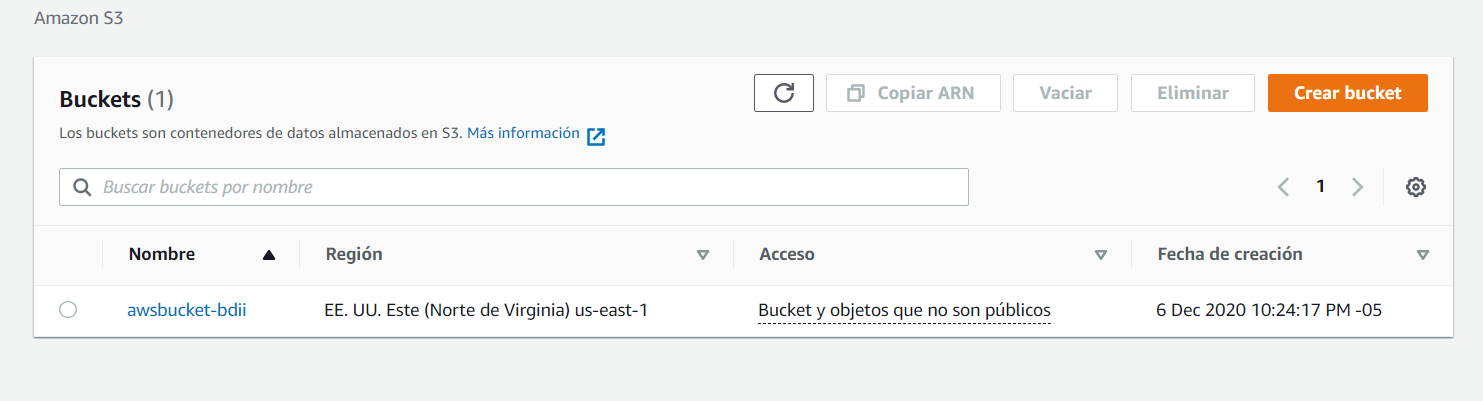
\includegraphics[width=15cm]{./images/4} 
	\end{center}
\newpage
\textbf{1.3. Crear un par de claves de Amazon EC2 
}

    \begin{center}
		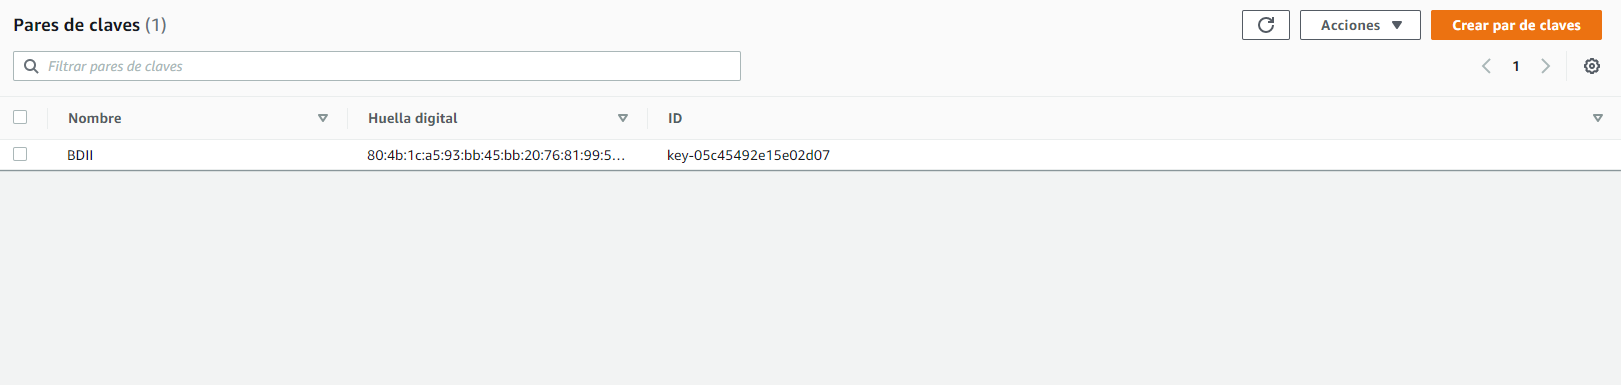
\includegraphics[width=15cm]{./images/5} 
	\end{center}

\section{Lanzar el clúster de Amazon EMR de ejemplo }

\textbf{2.1. Inicie sesión en la Consola de administración de AWS y abra la consola de Amazon EMR (https://
console.aws.amazon.com/elasticmapreduce/). }

    \begin{center}
		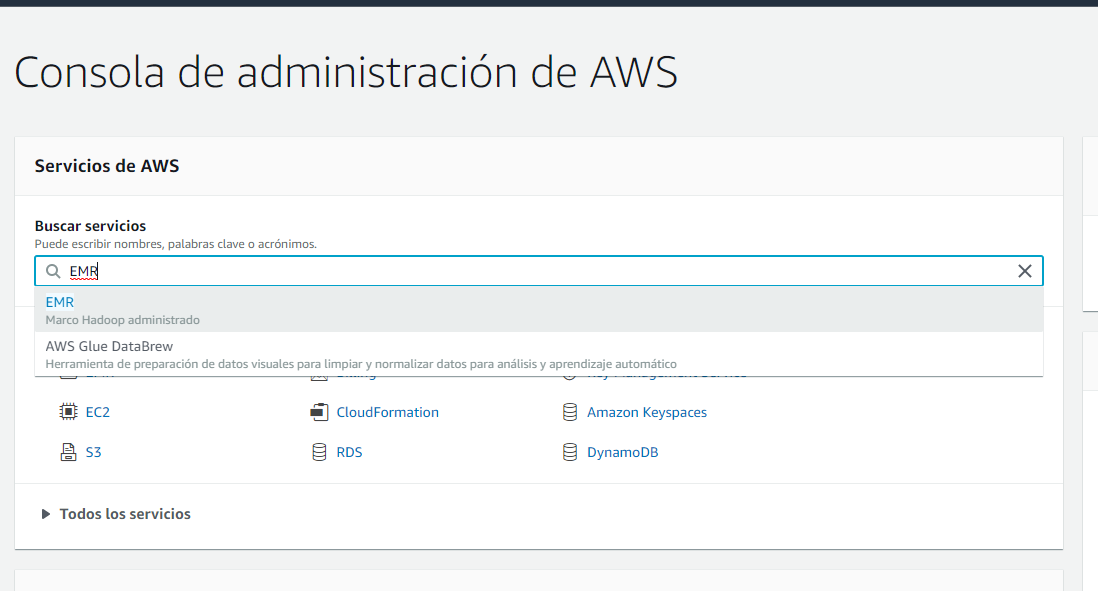
\includegraphics[width=15cm]{./images/6} 
	\end{center}
	\newpage
\textbf{2.2. Elija Create cluster (Crear clúster)}

    \begin{center}
		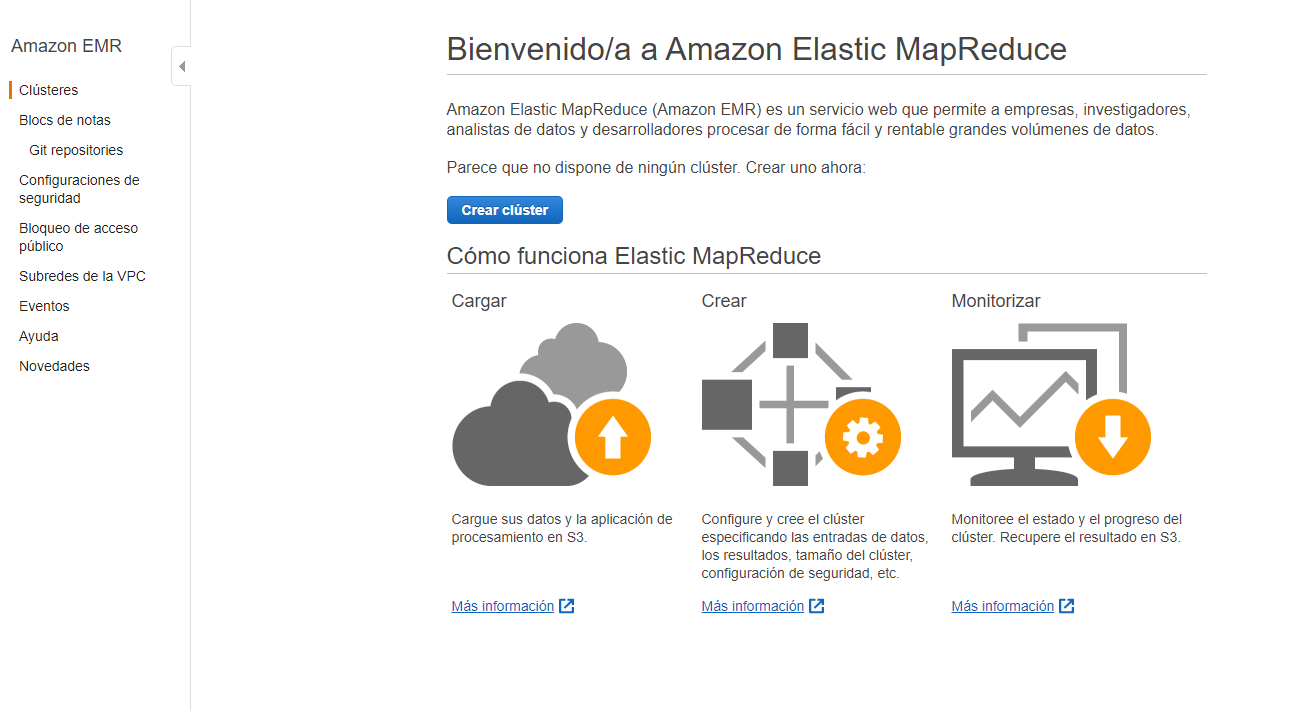
\includegraphics[width=15cm]{./images/7} 
	\end{center}
\newpage
\textbf{2.3. En la página Create Cluster - Quick Options (Crear clúster: opciones rápidas), acepte los valores
predeterminados
}

    \begin{center}
		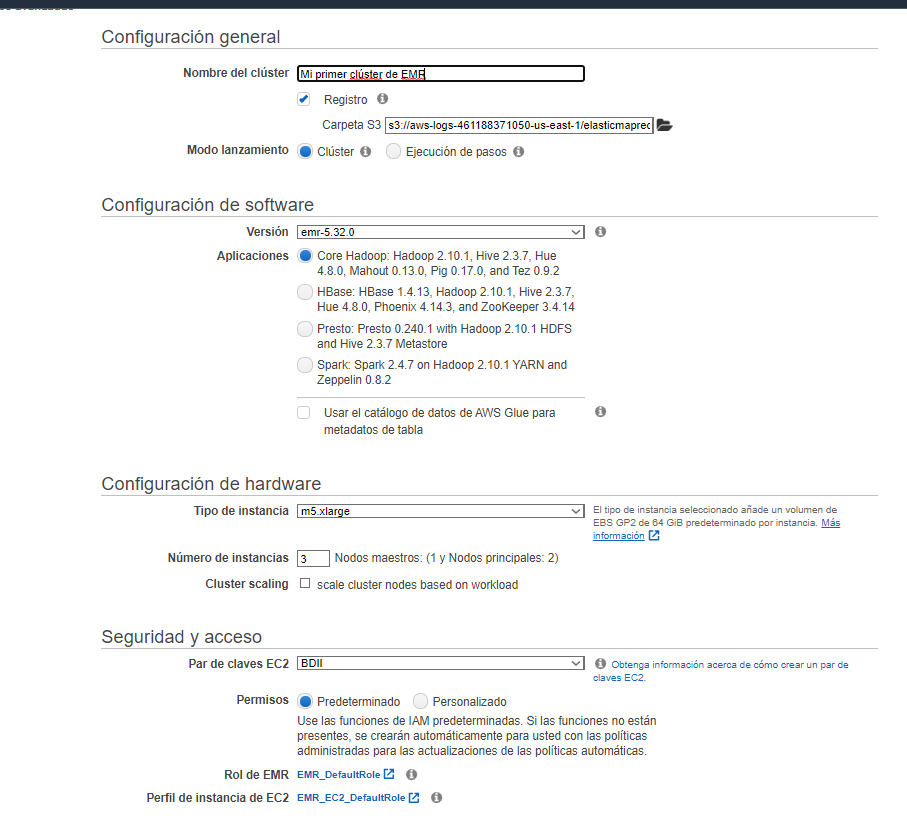
\includegraphics[width=15cm]{./images/8} 
	\end{center}

\newpage
\textbf{2.4. Elija Create cluster
}

    \begin{center}
		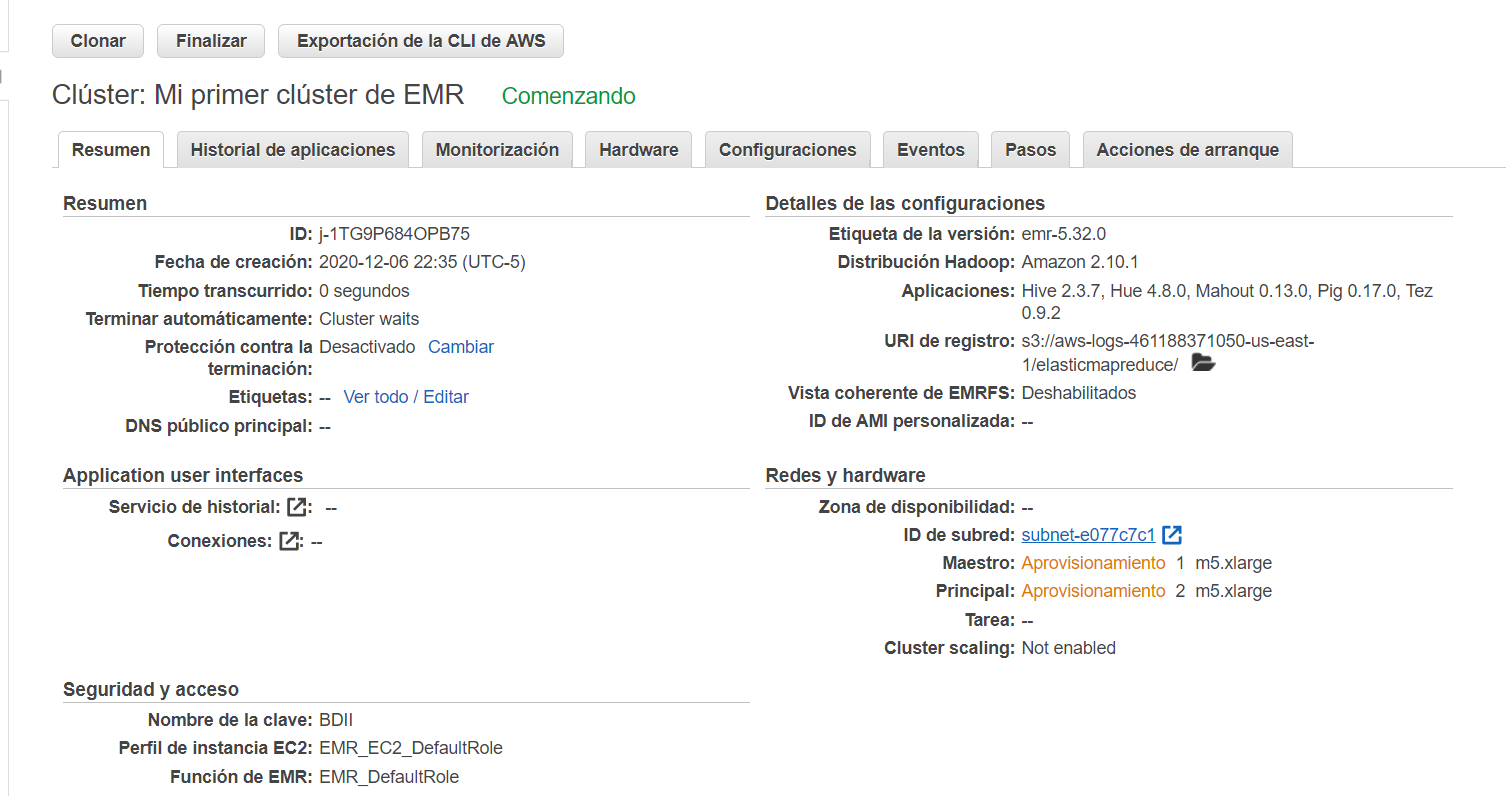
\includegraphics[width=15cm]{./images/9} 
	\end{center}


\section{Permitir las conexiones SSH con el clúster desde el cliente }

\textbf{3.1. Abra la consola de Amazon EMR en https://console.aws.amazon.com/elasticmapreduce/ }

    \begin{center}
		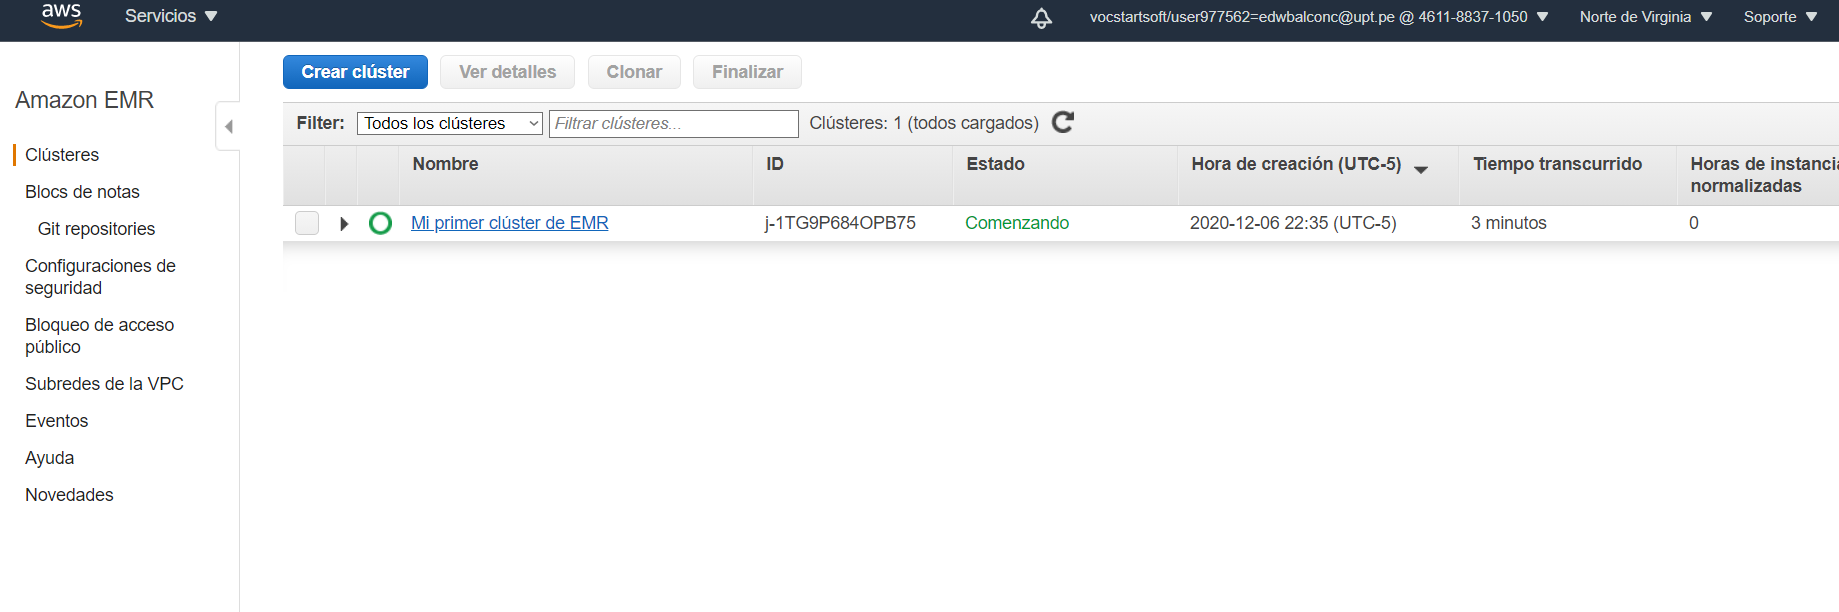
\includegraphics[width=15cm]{./images/10} 
	\end{center}
	\newpage
\textbf{3.2.Seleccione Clusters (Clústeres). }

    \begin{center}
		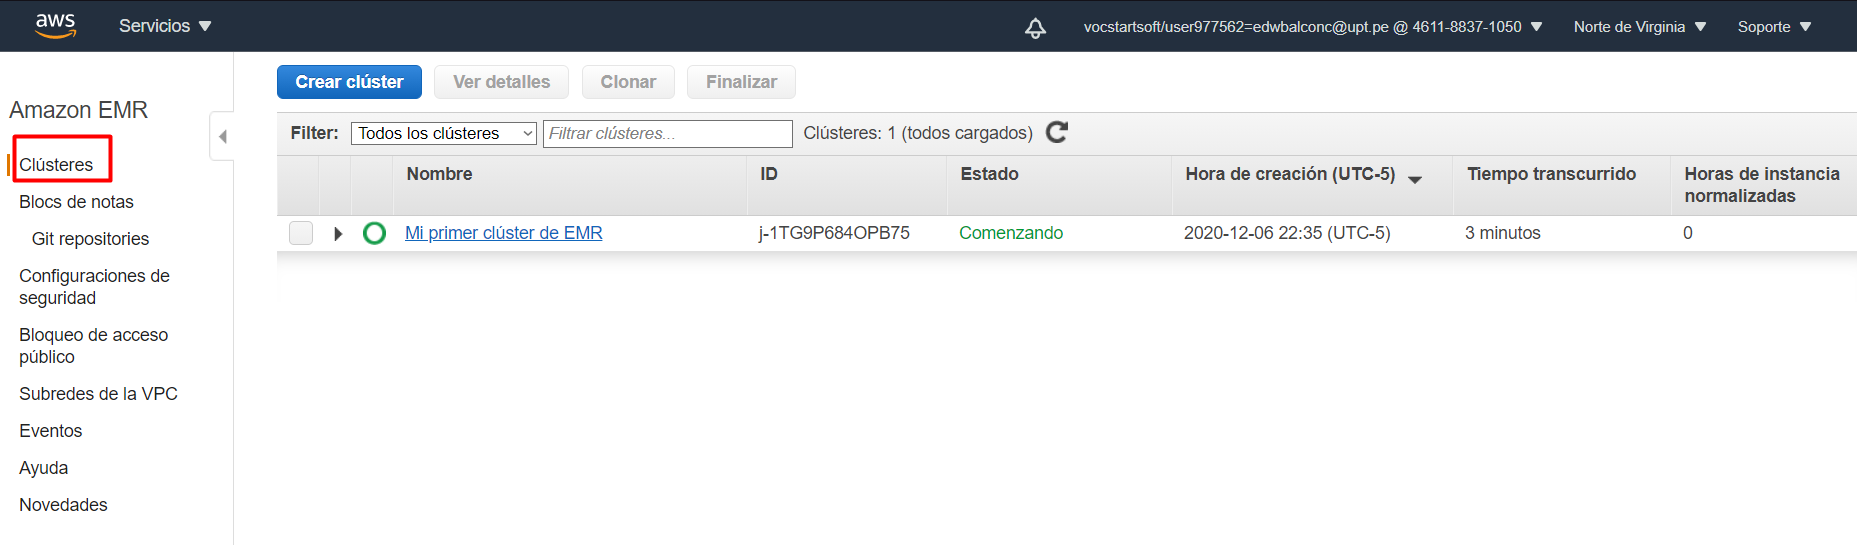
\includegraphics[width=15cm]{./images/11} 
	\end{center}
\textbf{3.3. Elija el Name (Nombre) del clúster. 
}

    \begin{center}
		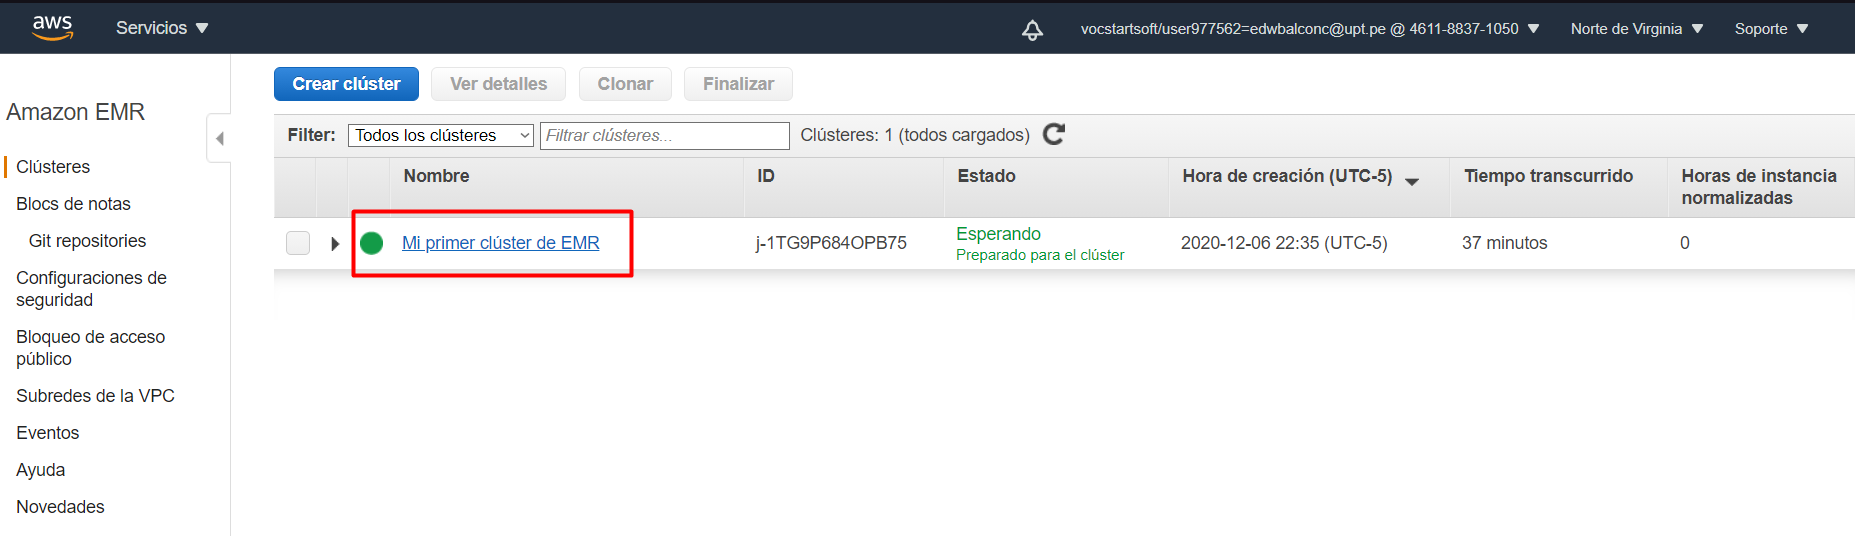
\includegraphics[width=15cm]{./images/12} 
	\end{center}

\newpage
\textbf{3.4. En Security and access (Seguridad y acceso), elija el enlace Security groups for Master (Grupos de
seguridad para principal).
}

    \begin{center}
		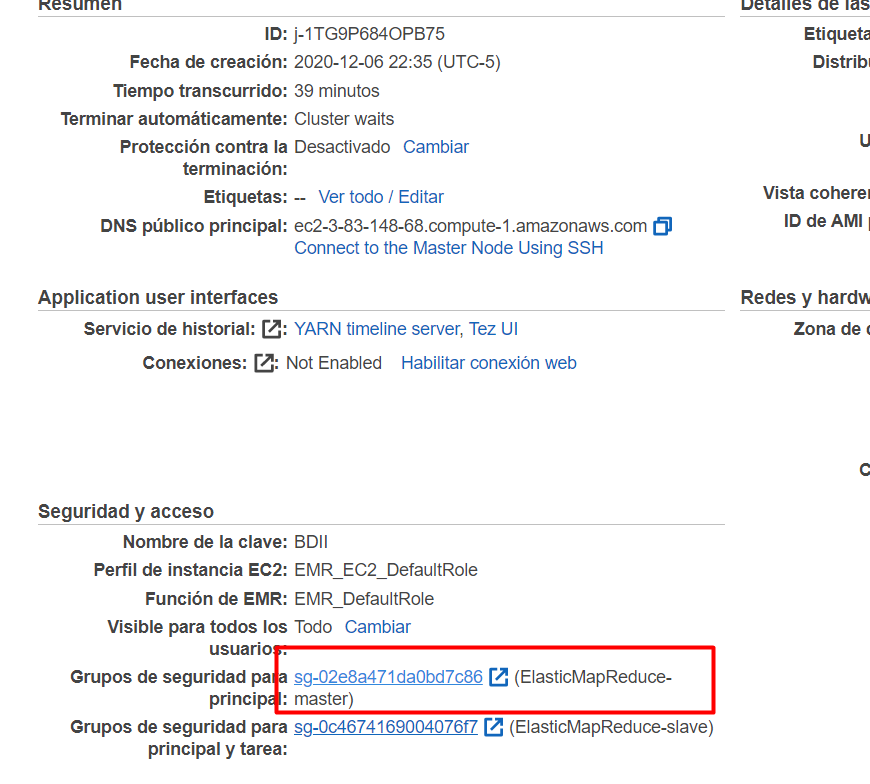
\includegraphics[width=15cm]{./images/13} 
	\end{center}

\newpage
\textbf{3.5. Elija ElasticMapReduce-master en la lista. 
}

    \begin{center}
		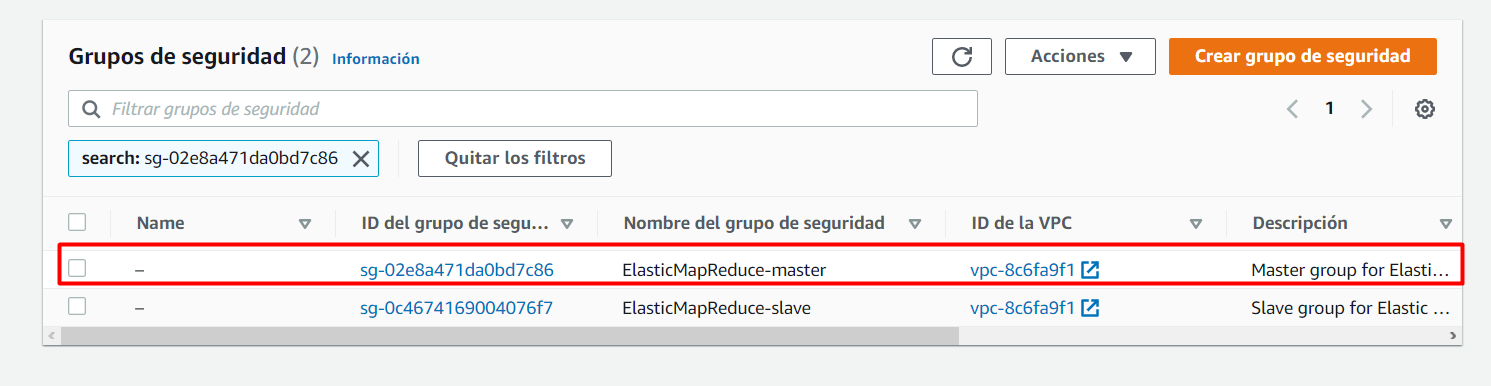
\includegraphics[width=15cm]{./images/14} 
	\end{center}
\textbf{3.6. Elija Inbound (Entrada), Edit (Editar). 
}

    \begin{center}
		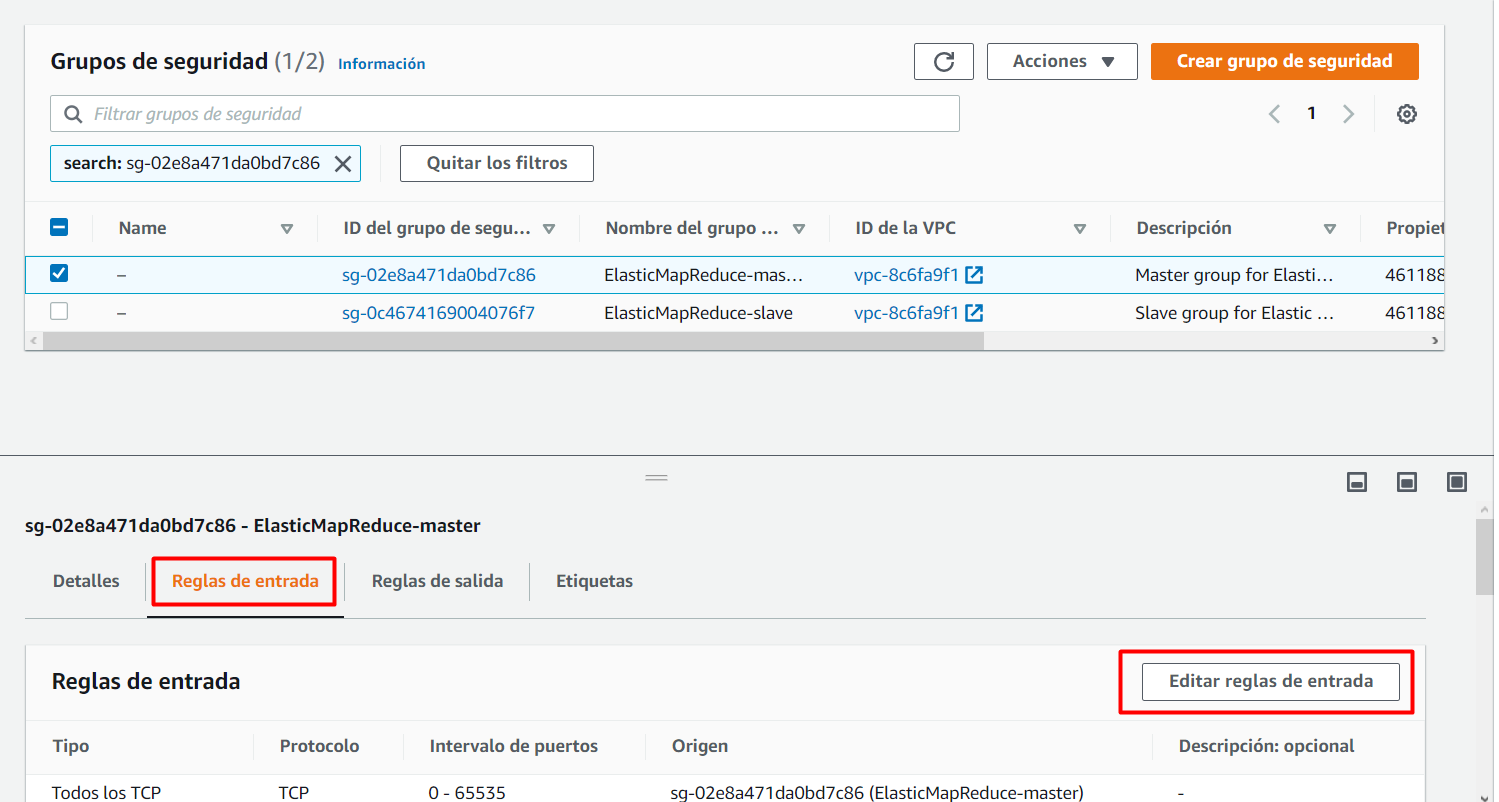
\includegraphics[width=15cm]{./images/15} 
	\end{center}


\newpage
\textbf{3.7. Compruebe si hay una regla de entrada que permite el acceso público con la siguiente configuración. Si
existe, elija Delete (Eliminar) para eliminarla
}

    \begin{center}
		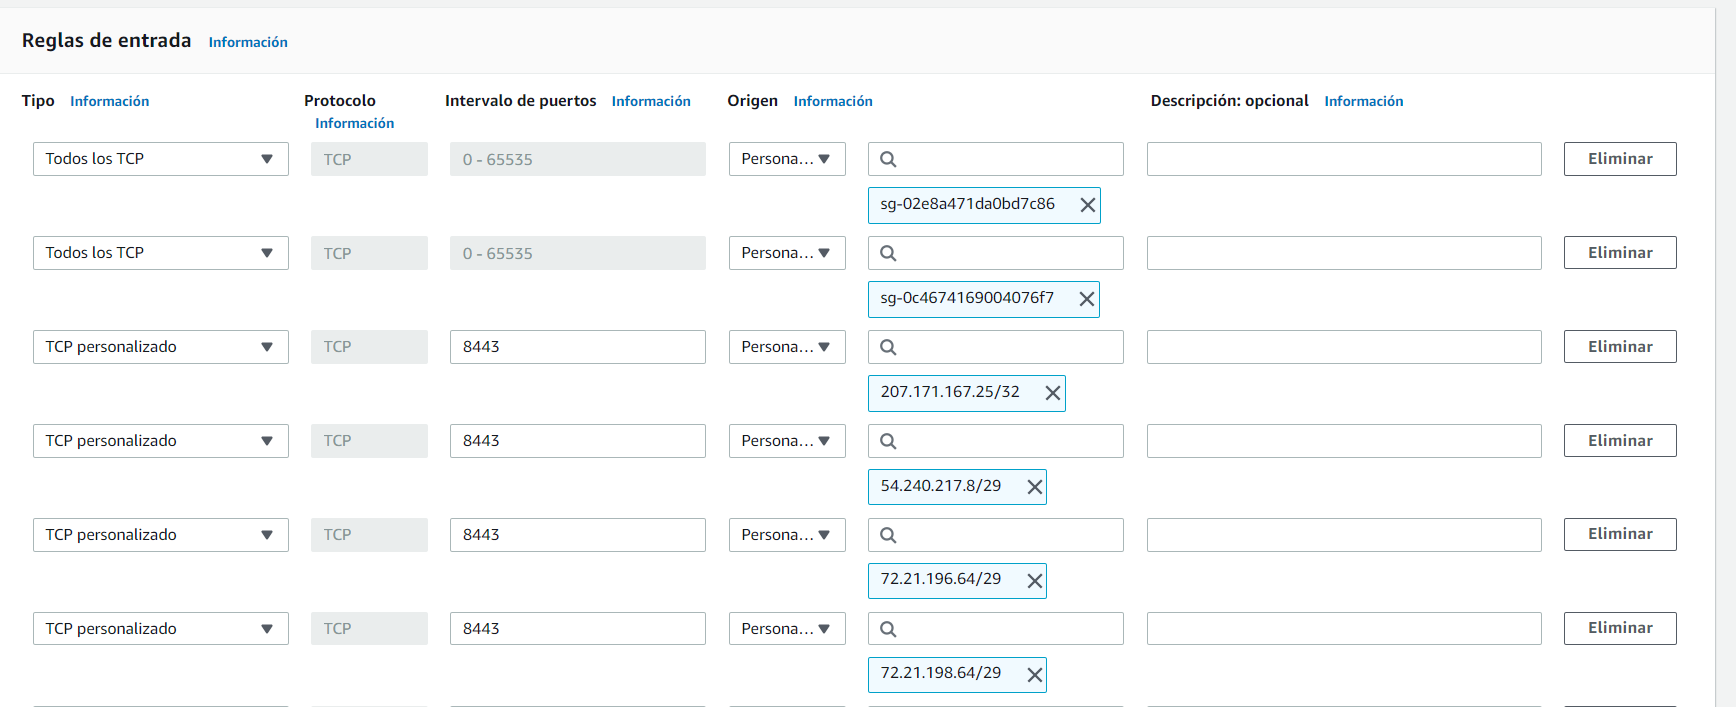
\includegraphics[width=15cm]{./images/16} 
	\end{center}



\textbf{3.8. Desplácese a la parte inferior de la lista y elija Add Rule (Añadir regla). 
}

    \begin{center}
		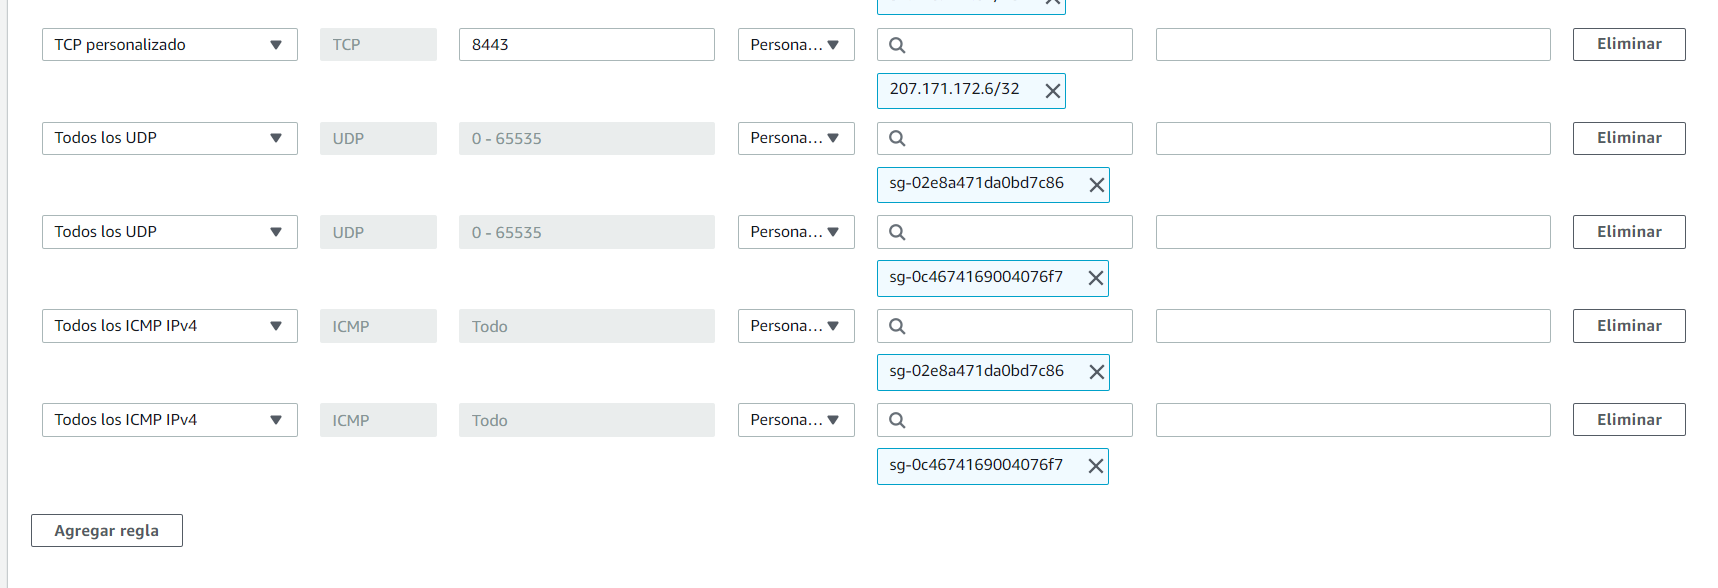
\includegraphics[width=15cm]{./images/17} 
	\end{center}

\newpage
\textbf{3.9. En Type (Tipo), seleccione SSH. Esto introduce automáticamente TCP para Protocol (Protocolo) y 22
para Port Range (Rango de puertos). 
}

    \begin{center}
		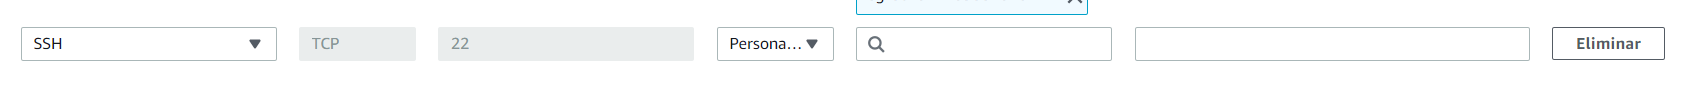
\includegraphics[width=15cm]{./images/18} 
	\end{center}

\textbf{3.10. Como origen, seleccione My IP (Mi IP). Esto añade automáticamente la dirección IP del equipo cliente
como la dirección de origen. También puede añadir un rango de direcciones IP de clientes de confianza
Custom (Personalizadas) y elegir Add rule (Añadir regla) para crear reglas adicionales para otros
clientes. Muchos entornos de red asignan dinámicamente direcciones IP, por lo que es posible que 
necesite editar periódicamente las reglas de grupos de seguridad para actualizar las direcciones IP de
los clientes de confianza. 
}

    \begin{center}
		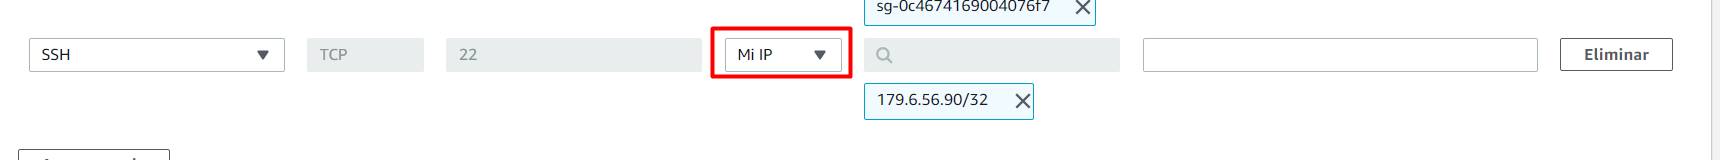
\includegraphics[width=15cm]{./images/19} 
	\end{center}


\textbf{3.11. Elija Save (Guardar).
}

    \begin{center}
		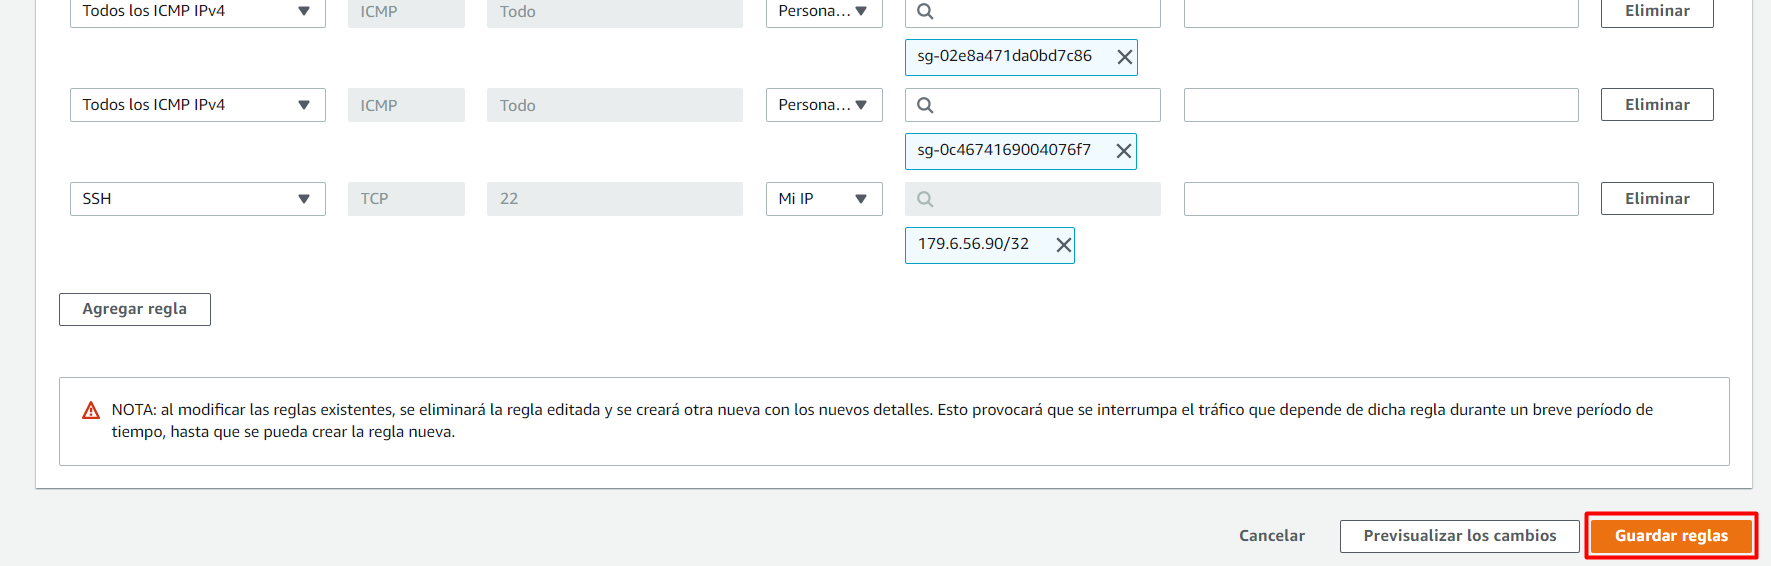
\includegraphics[width=15cm]{./images/20} 
	\end{center}
\newpage

\section{Procesar los datos ejecutando el script de Hive como paso }

\textbf{4.1. Abra la consola de Amazon EMR en https://console.aws.amazon.com/elasticmapreduce/ }

    \begin{center}
		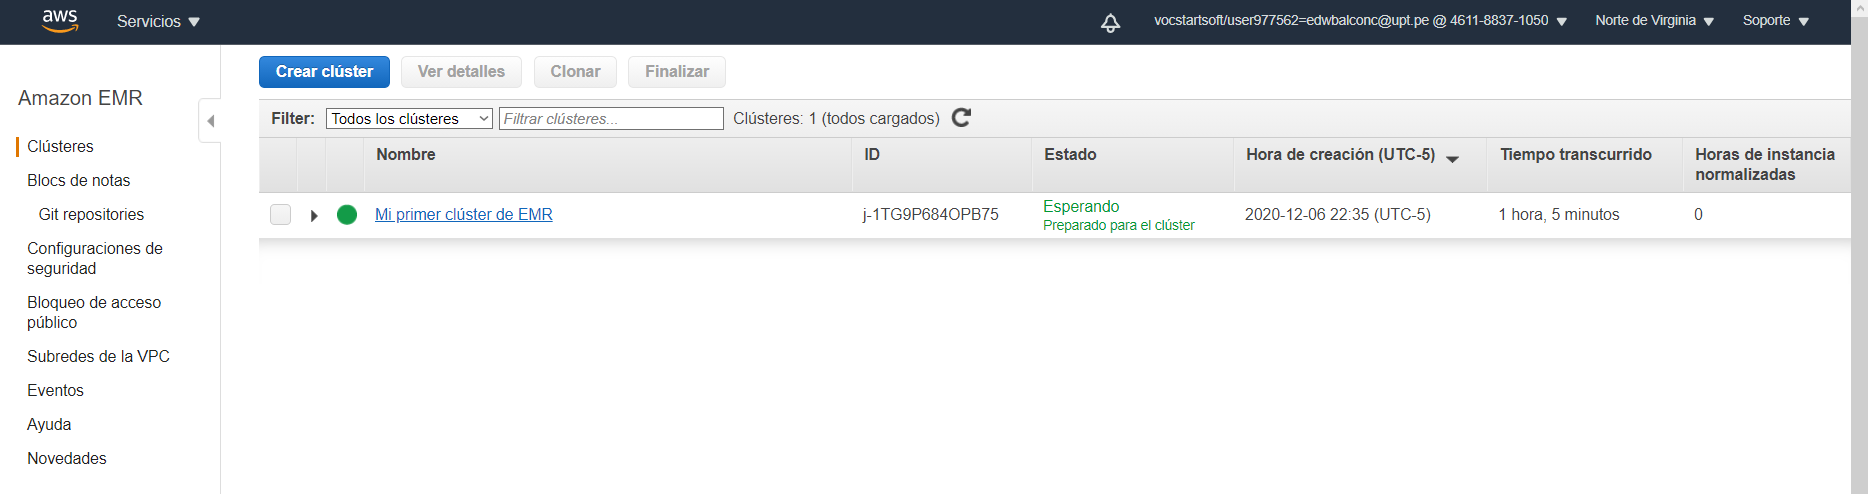
\includegraphics[width=15cm]{./images/21} 
	\end{center}
\textbf{4.2.En Cluster List (Lista de clústeres), seleccione el nombre del clúster. Asegúrese de que el clúster está en
el estado Waiting (Esperando).  }

    \begin{center}
		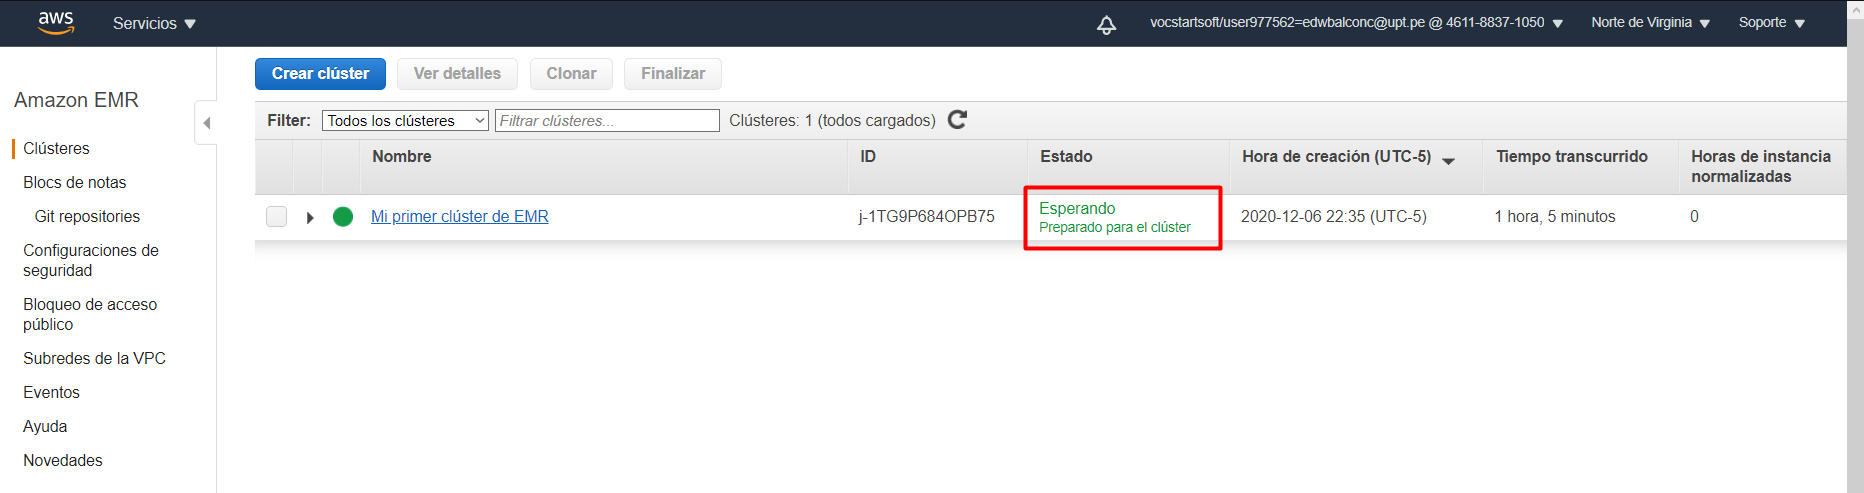
\includegraphics[width=15cm]{./images/22} 
	\end{center}
	\newpage
\textbf{4.3.Elija Steps (Pasos) y, a continuación Add step (Añadir paso). 
}

    \begin{center}
		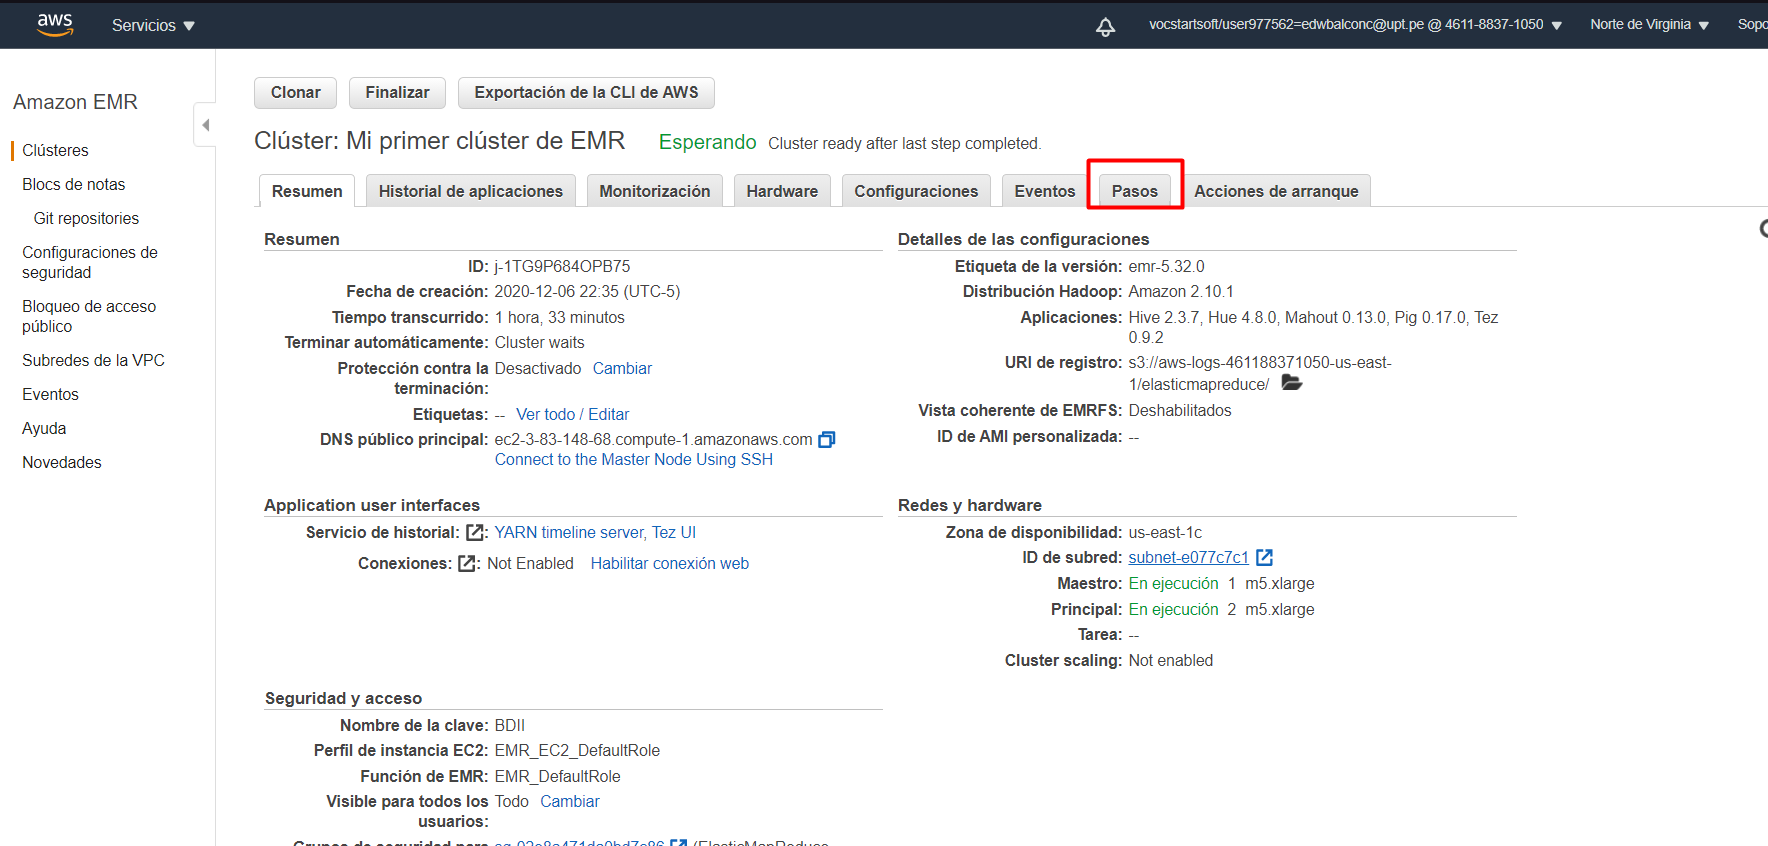
\includegraphics[width=15cm]{./images/23} 
	\end{center}

\textbf{4.4. Configure el paso de acuerdo con las directrices siguientes:
}

    \begin{center}
		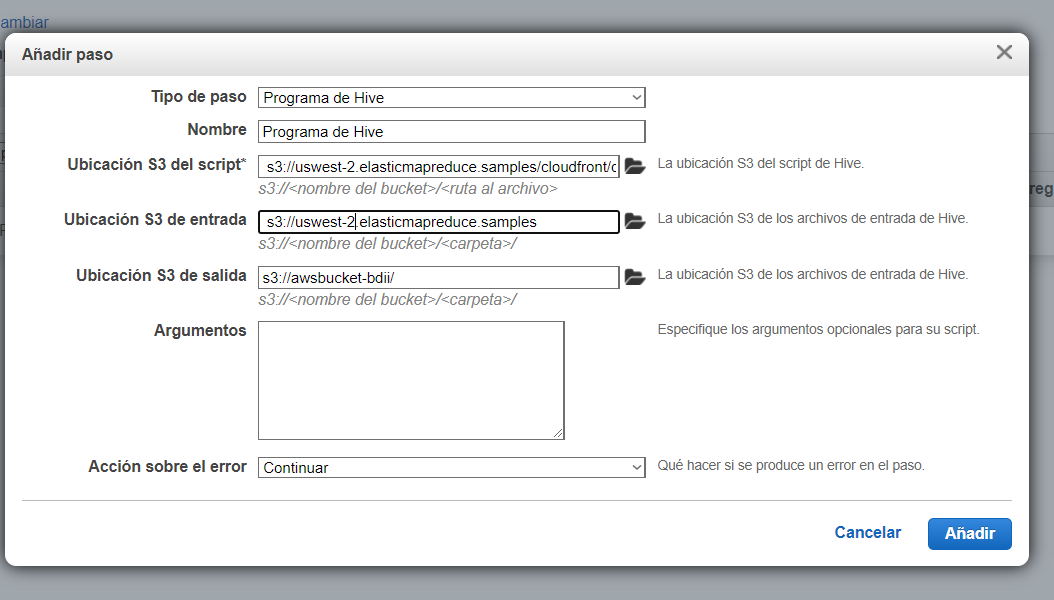
\includegraphics[width=15cm]{./images/24} 
	\end{center}

\newpage
\textbf{4.5. Elija Add (Añadir). El paso aparece en la consola con el estado Pending (Pendiente). 
}

    \begin{center}
		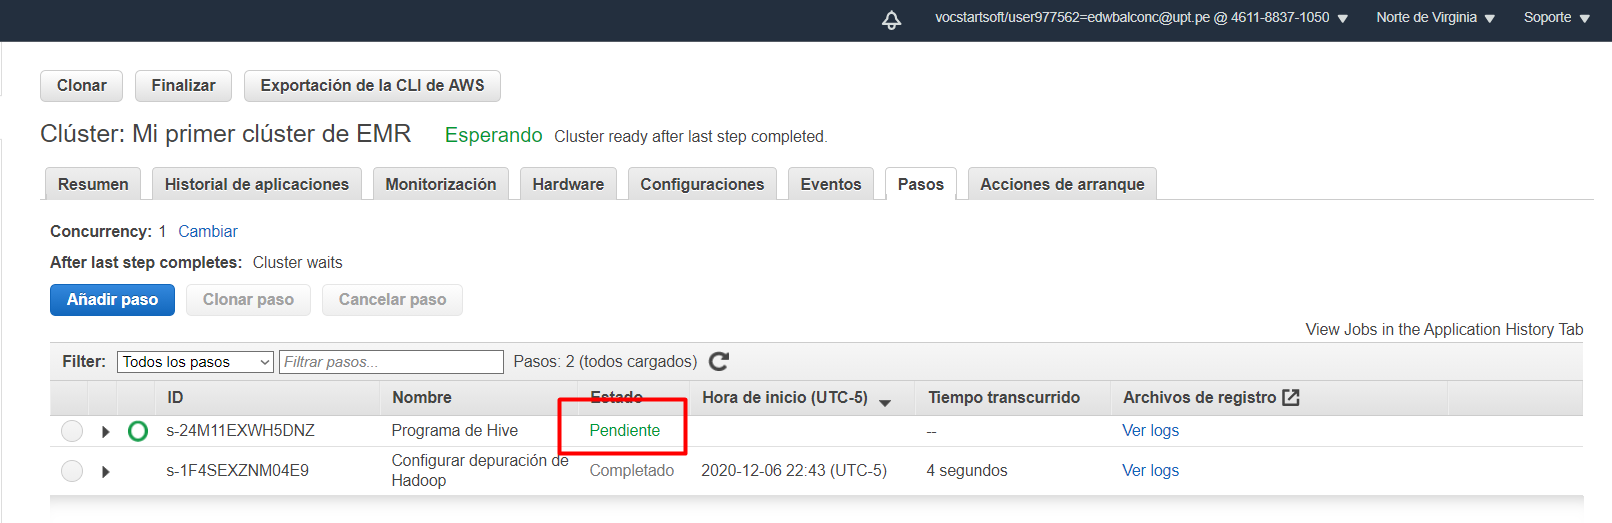
\includegraphics[width=15cm]{./images/25} 
	\end{center}
\textbf{4.6. El estado del paso cambia de Pending (Pendiente) a Running (En ejecución) y a Completed
(Completado) a medida que se ejecuta. Para actualizar el estado, elija el icono de actualización situado
a la derecha de Filter (Filtro). El script tarda aproximadamente un minuto en ejecutarse. 
}

    \begin{center}
		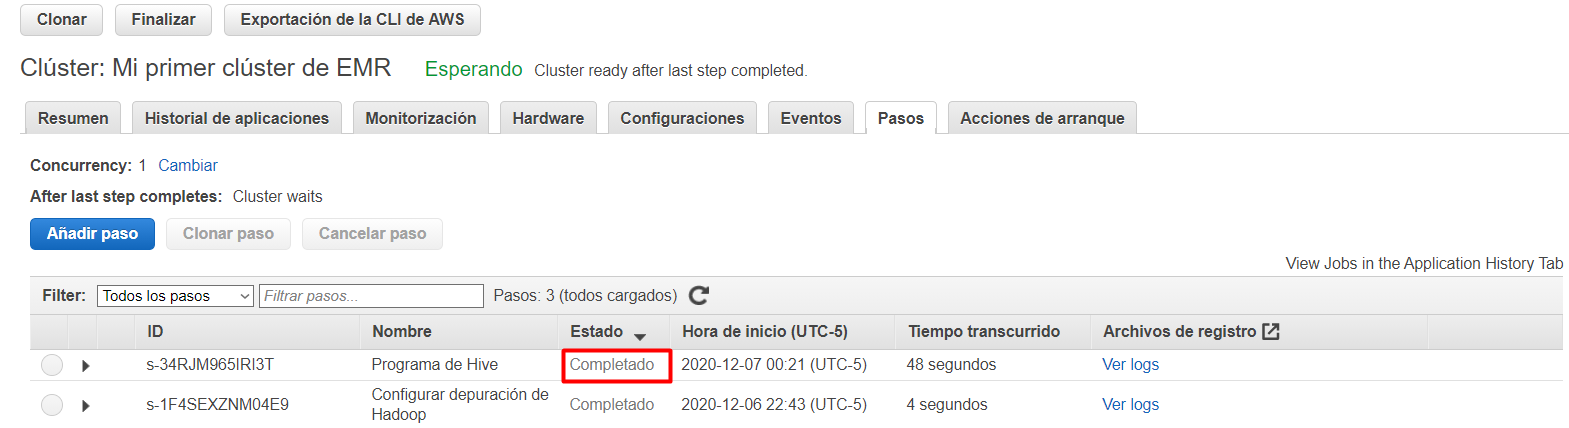
\includegraphics[width=15cm]{./images/26} 
	\end{center}


\newpage

\section{Ver los resultados Una vez que el paso se completa correctamente }

\textbf{5.1. Abra la consola de Amazon S3 en https://console.aws.amazon.com/s3/. }

    \begin{center}
		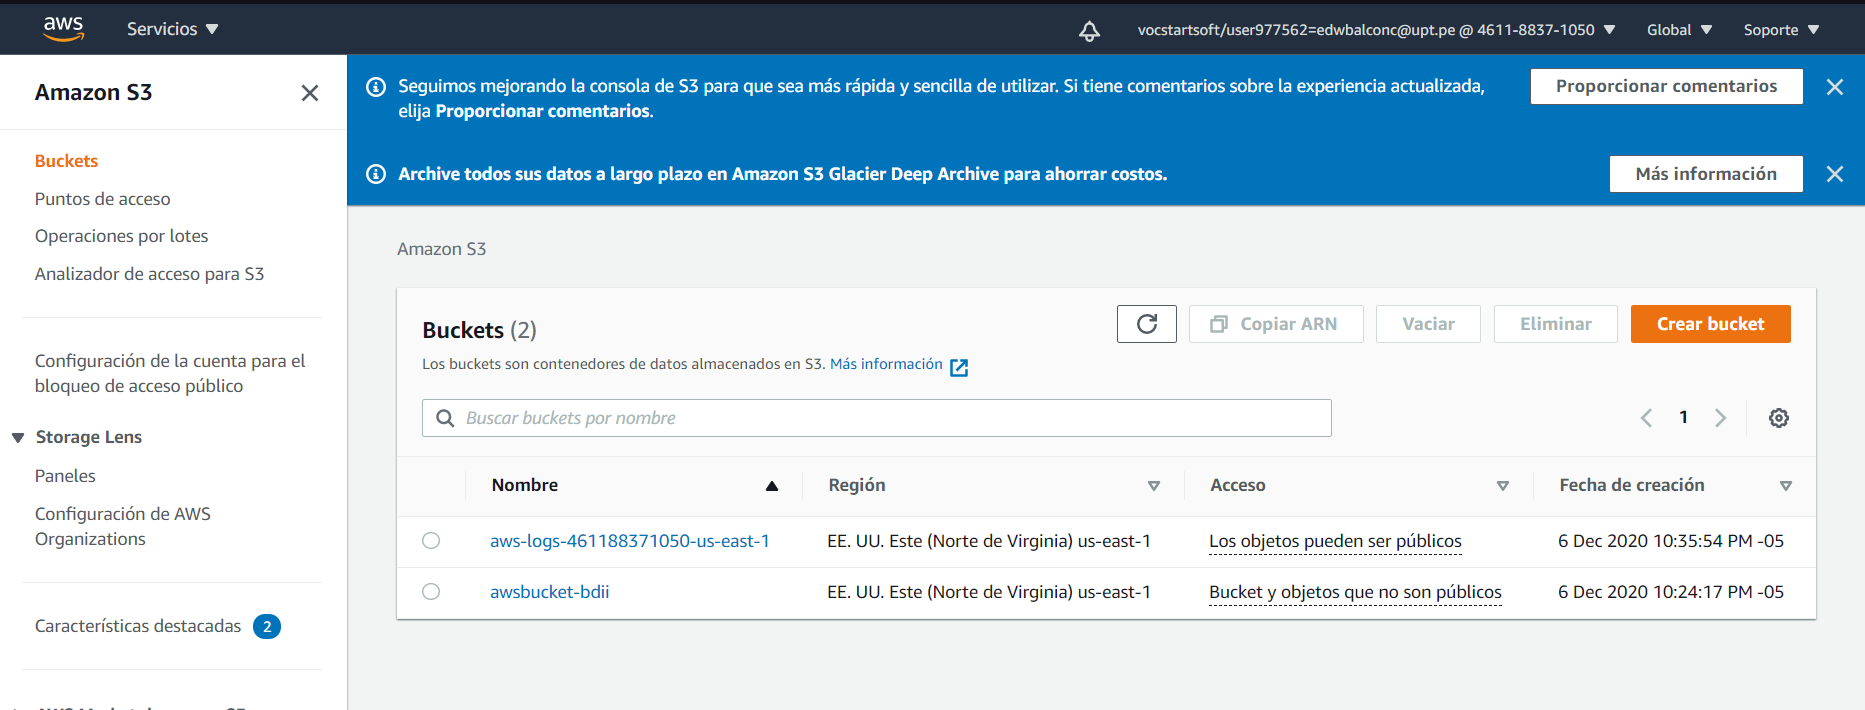
\includegraphics[width=15cm]{./images/27} 
	\end{center}
\textbf{5.2.Elija el Bucket name (Nombre del bucket) y, a continuación, elija la carpeta que ha configurado
anteriormente. Por ejemplo, mybucket y luego MyHiveQueryResults.   }

    \begin{center}
		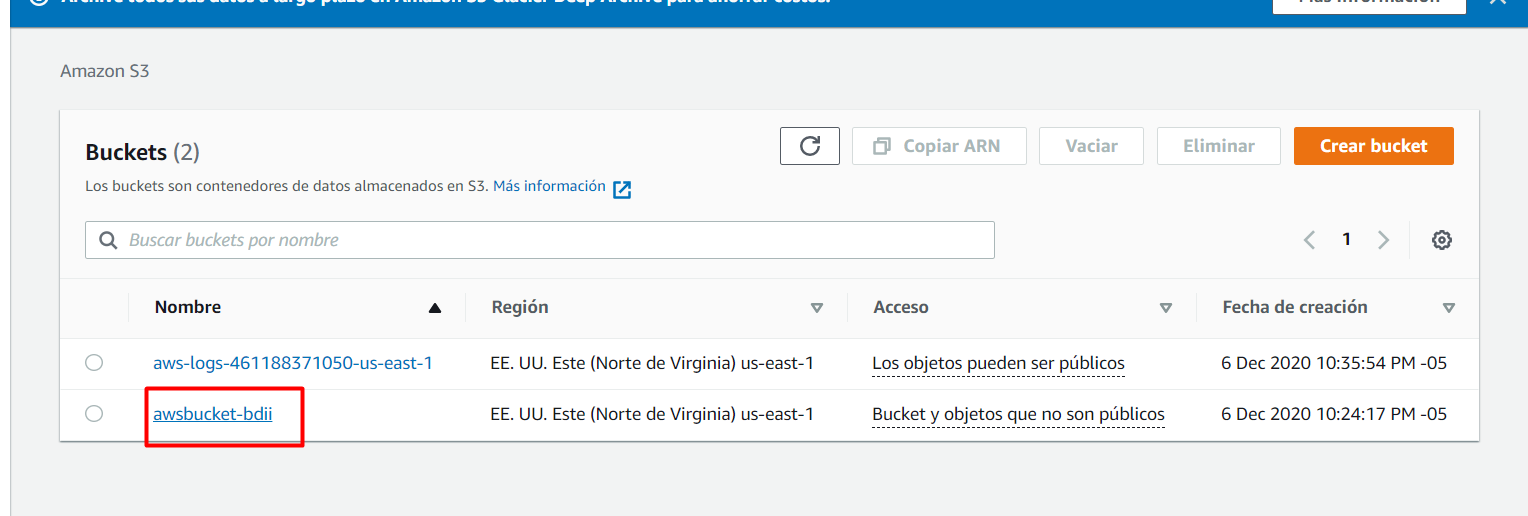
\includegraphics[width=15cm]{./images/28} 
	\end{center}
	\newpage
\textbf{5.3.La consulta escribe los resultados en una carpeta ubicada en la carpeta de salida denominada
os_requests. Elija esa carpeta. Debería haber un único archivo denominado 000000_0 en dicha
carpeta. Se trata de un archivo de texto que contiene los resultados de la consulta de Hive. 
}

    \begin{center}
		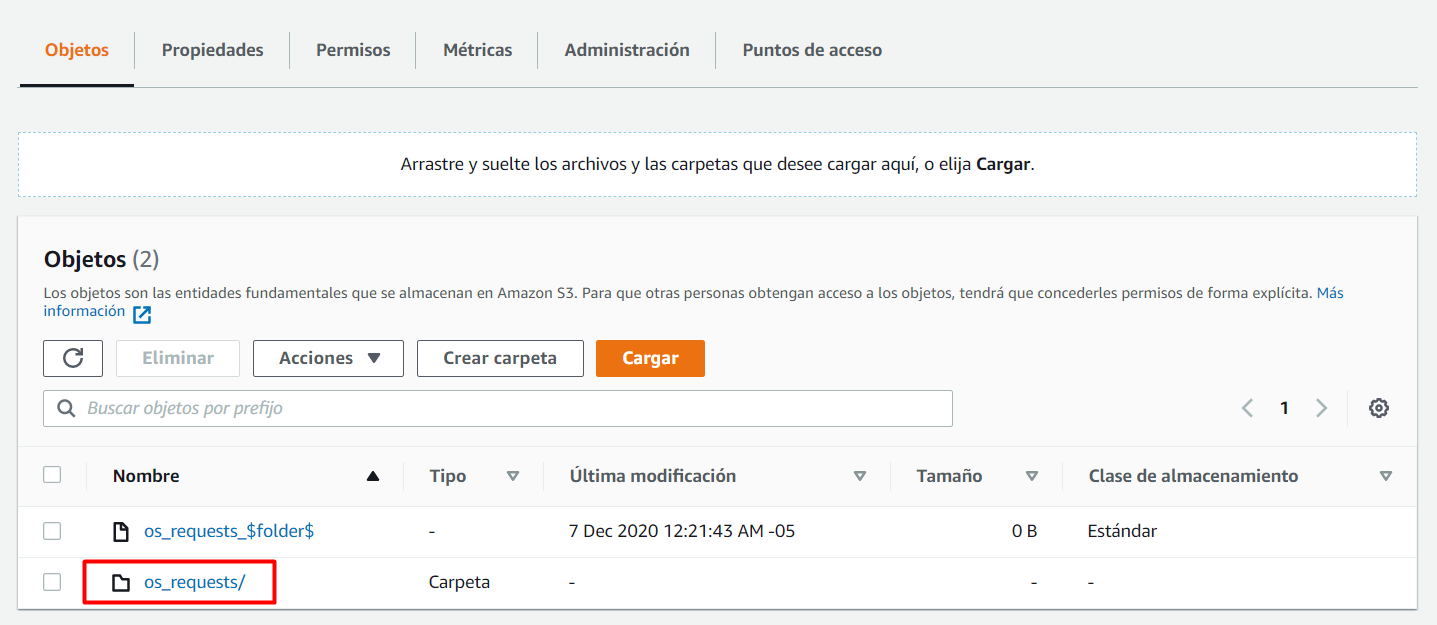
\includegraphics[width=15cm]{./images/29} 
	\end{center}

\textbf{5.4. Elija el archivo y, a continuación, elija Download (Descargar) para guardarlo localmente. 
}

    \begin{center}
		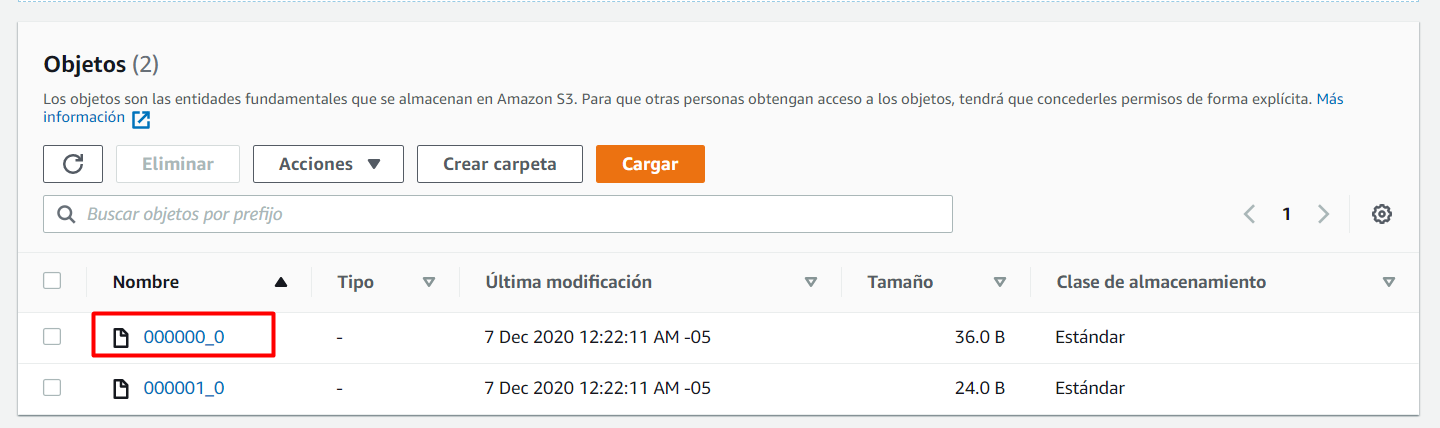
\includegraphics[width=15cm]{./images/30} 
	\end{center}

\begin{center}
		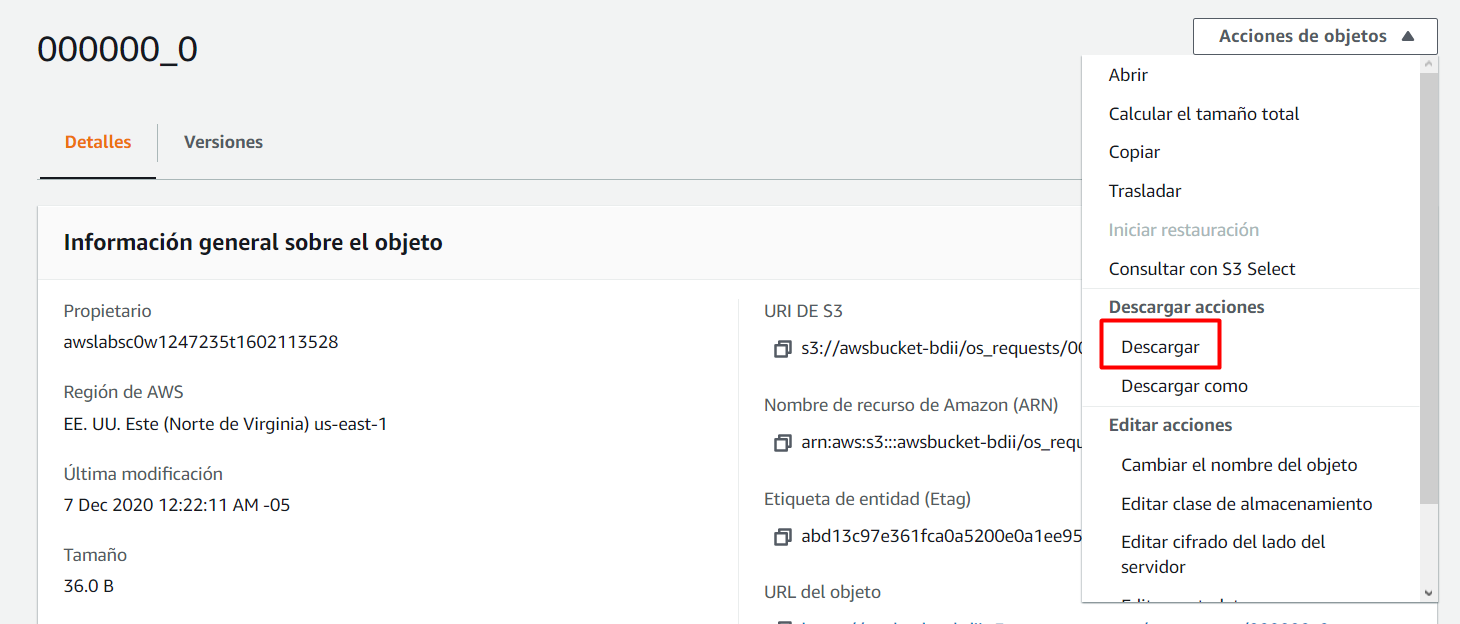
\includegraphics[width=15cm]{./images/31} 
	\end{center}
\textbf{5.5. Utilice el editor de texto que prefiera para abrir el archivo. El archivo de salida muestra el número
de solicitudes de acceso ordenadas por sistema operativo. El siguiente ejemplo muestra la salida en
WordPad:
}

    \begin{center}
		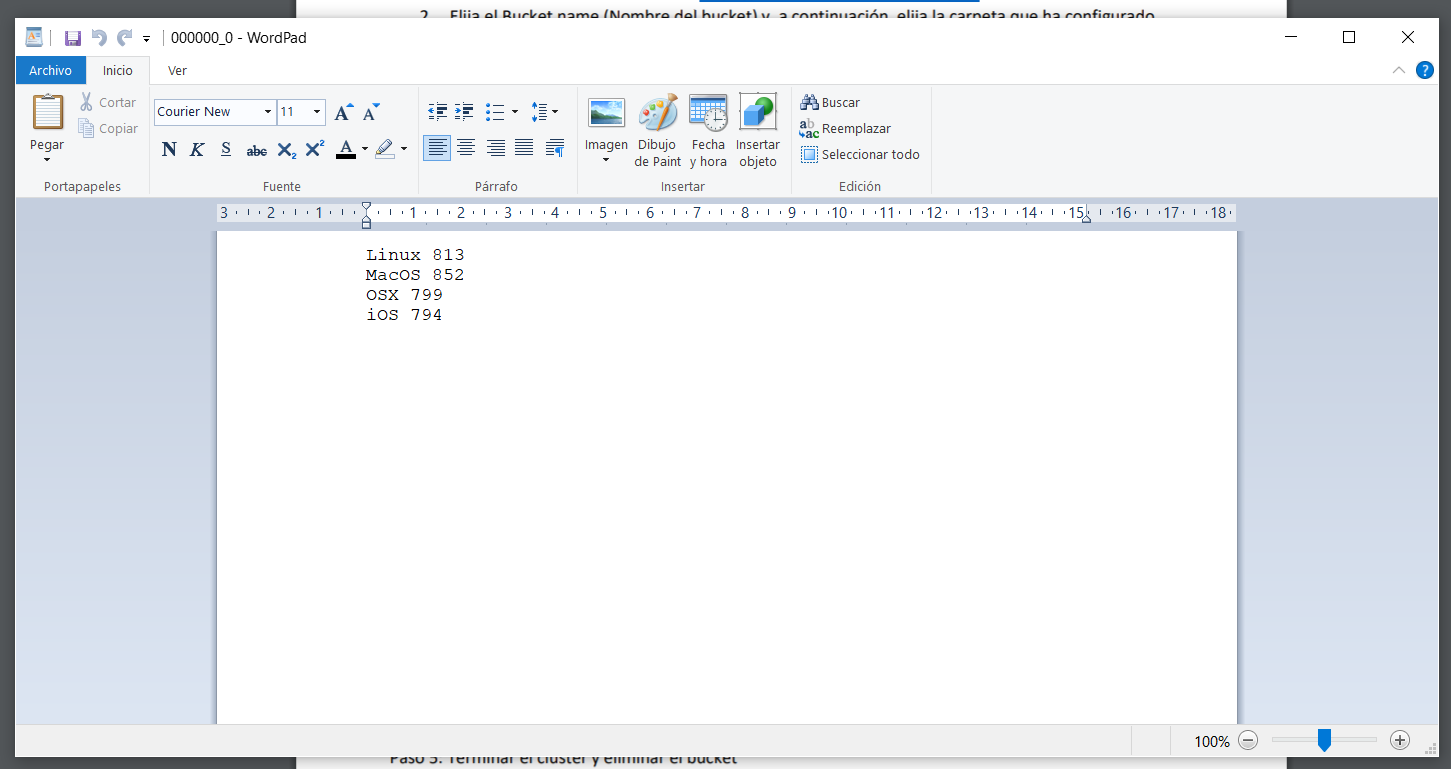
\includegraphics[width=15cm]{./images/32} 
	\end{center}

\newpage

\section{ Terminar el clúster y eliminar el bucket  }

\textbf{6.1. Abra la consola de Amazon EMR en https://console.aws.amazon.com/elasticmapreduce/.  }

    \begin{center}
		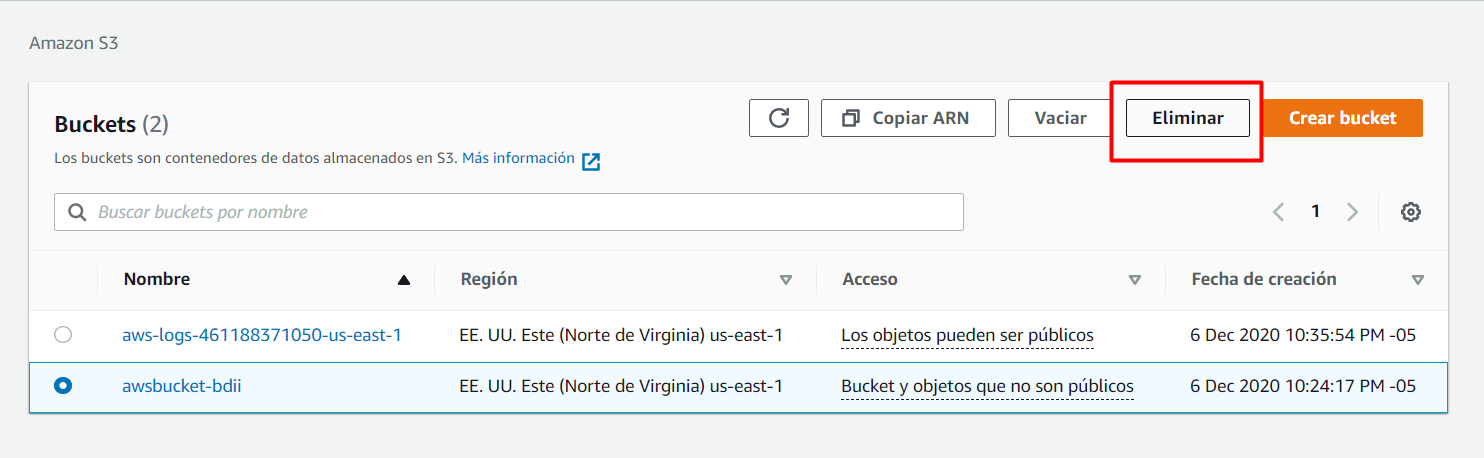
\includegraphics[width=15cm]{./images/33} 
	\end{center}
6\textbf{6.2.Elija Clusters (Clústeres), elija el clúster y, a continuación, Terminate (Terminar).
Los clústeres suelen crearse con la protección de terminación activada, lo que ayuda a evitar que se
cierren de forma accidental. Si ha seguido el tutorial al pie de la letra, la protección de terminación
debería estar desactivada. Si la protección de terminación está activada, se le pedirá que cambie esta
opción como medida de precaución antes de terminar el clúster. Elija Change (Cambiar), Off
(Desactivada).   }

    \begin{center}
		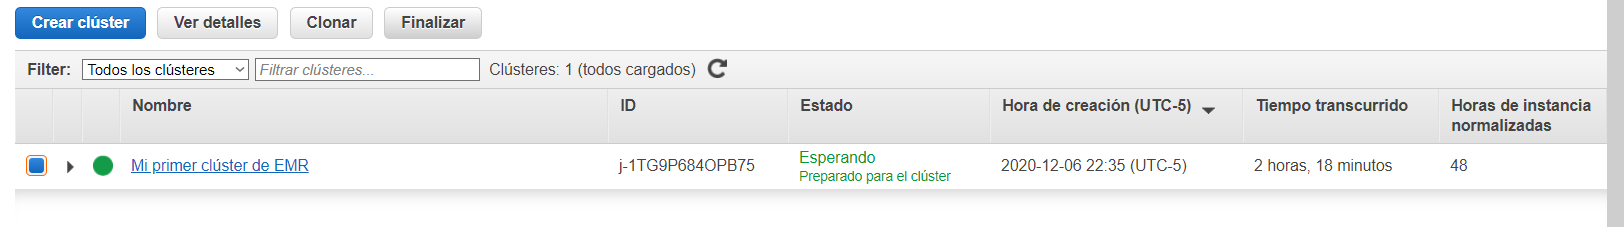
\includegraphics[width=15cm]{./images/34} 
	\end{center}

\end{document}